\subsection{Audio-Schaltung}
\label{subsec:Audio-Schaltung}

Für die Validierung des Analog-Teils wurden verschiedene Teil-Messungen durchgeführt welche nachfolgend erklärt werden.

\subsubsection{Frequenzgang}
\label{subsubsec:Frequenzgang}
Um zu beurteilen ob die Audio-Wandlung und Rückwandlung korrekt funktioniert wird der Frequenzgang der entworfenen Schaltung gemessen. Damit sollte ersichtlich werden welche Frequenz mit welcher Verstärkung von Ein- zu Ausgang übertragen wird. Angestrebt wäre eine möglichst linearer Frequenzgang mit einer Verstärkung von 1 (0dB) auf allen Frequenzen.

\textbf{Anmerkung:} Da am Line-Eingang ein Spannungsteiler die Amplitude des Signals halbiert wurde dies software-mässig korrigiert. Das heisst 0dB in der Software bewirkt eigentlich +6dB am Codec, aber wiederum 0dB auf die ganze Schaltung gesehen wegen des Spannungsteilers.

\begin{figure} [H]
\begin{center}
 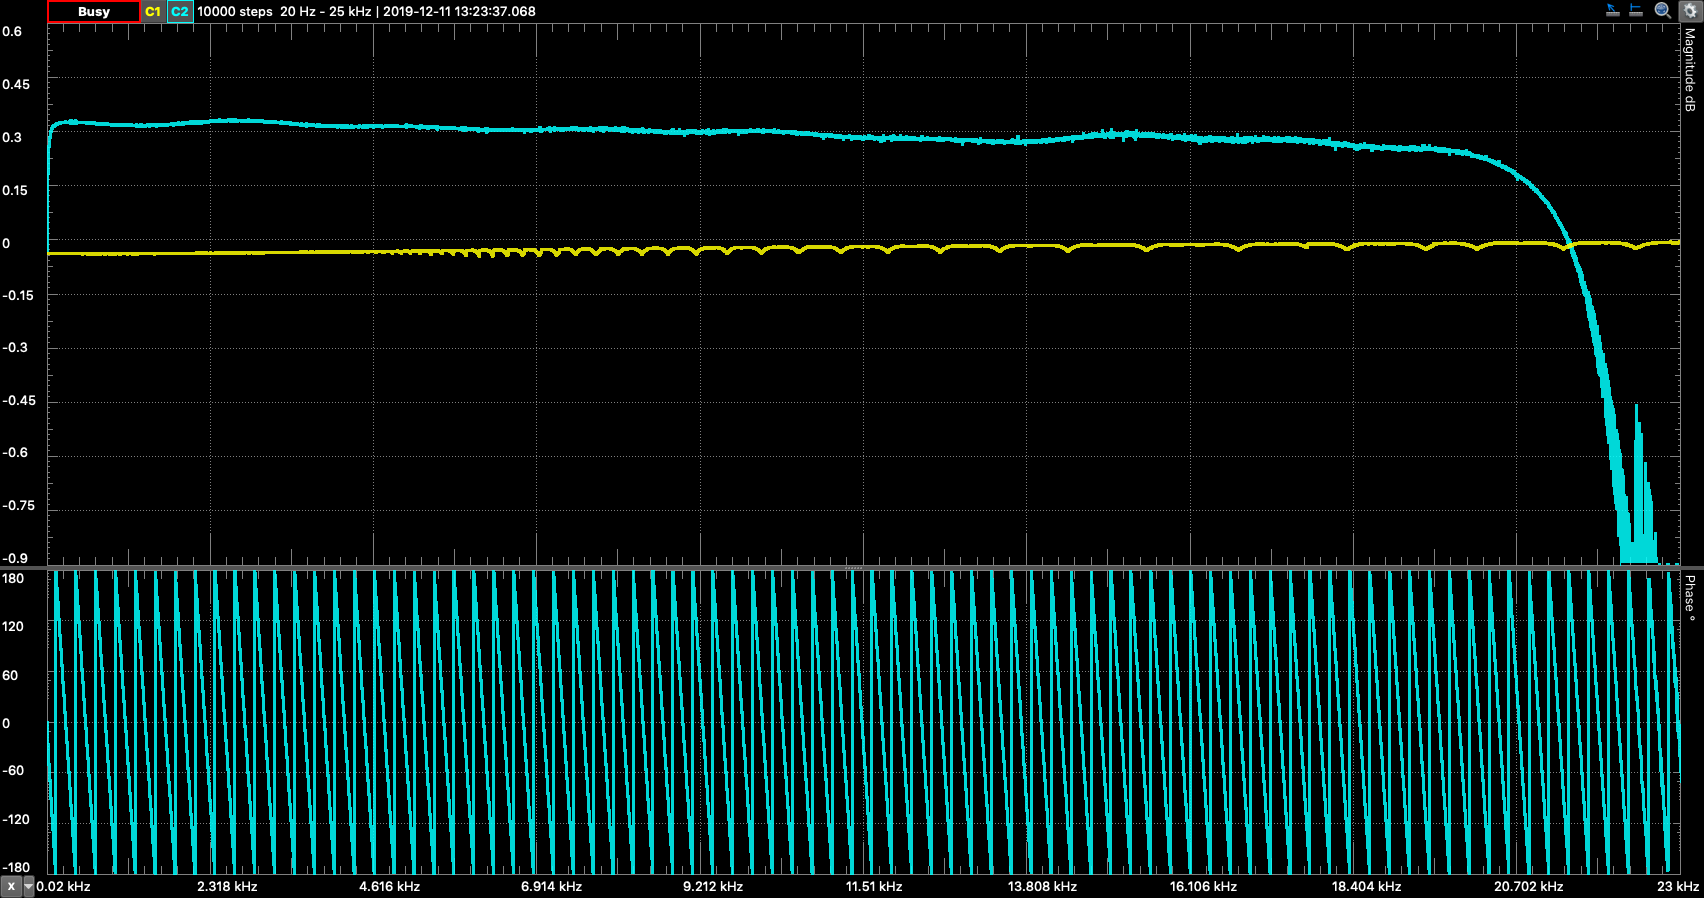
\includegraphics[width=\textwidth]{../graphics/FREQ_LineINOUT.png}
 \caption{Der gemessene Frequenzgang von Audio-Eingang zu Audio-Ausgang (oben) sowie der Phasengang der Schaltung(unten)}
\label{fig:frequenzgang}
\end{center}
\end{figure}
Die Messung wurde mit einem Analog Discovery 2 von Digilent durchgeführt. Der Netzwerk-Analyzer des AD2 generiert hierzu selbst einen Frequenz-Sweep. In \ref{fig:frequenzgang} sieht man das Referenz-Signal (gelb) im Vergleich zur Antwort durch die Schaltung (blau). Wie zu erwarten fängt das Anti-Aliasing-Filter bei der halben Abtastfrequenz (22.05kHz) an zu sperren. Der Phasengang ist wie erwartet linear mit entsprechenden Wrap-around von -180° zu 180°.
Offensichtlich verstärkt die Schaltung um ca. 0.3dB was ein Faktor 1.035 ist. Dies könnte von Wandlungs-Ungenaugkeiten des Codecs herrühren.

\subsubsection{Total Harmonic Distortion}
\label{subsubsec:Total Harmonic Distortion}
Die Total Harmonic Distortion oder auch THD genannt ist ein Leistungs-Verhältnis der harmonischen Oberschwingungen zum ursprünglich  eingespeisten Signal. In diesem Fall ist das eine Sinusschwingung mit einer Frequenz von 1kHz und $2V_{PP}$ Amplitude (generiert mit einem Agilent 33220A Waveform Generator). Das Signal wird am Eingang eingespiesen, wird einmal AD gewandelt, im Microcontroller 1zu1 kopiert und wieder zurückgewandelt. Am Ausgang wird nun die Amplitudde des Signals im Verhältnis zu dessen harmonischen Vielfachen gemessen.

\begin{figure} [H]
\begin{center}
 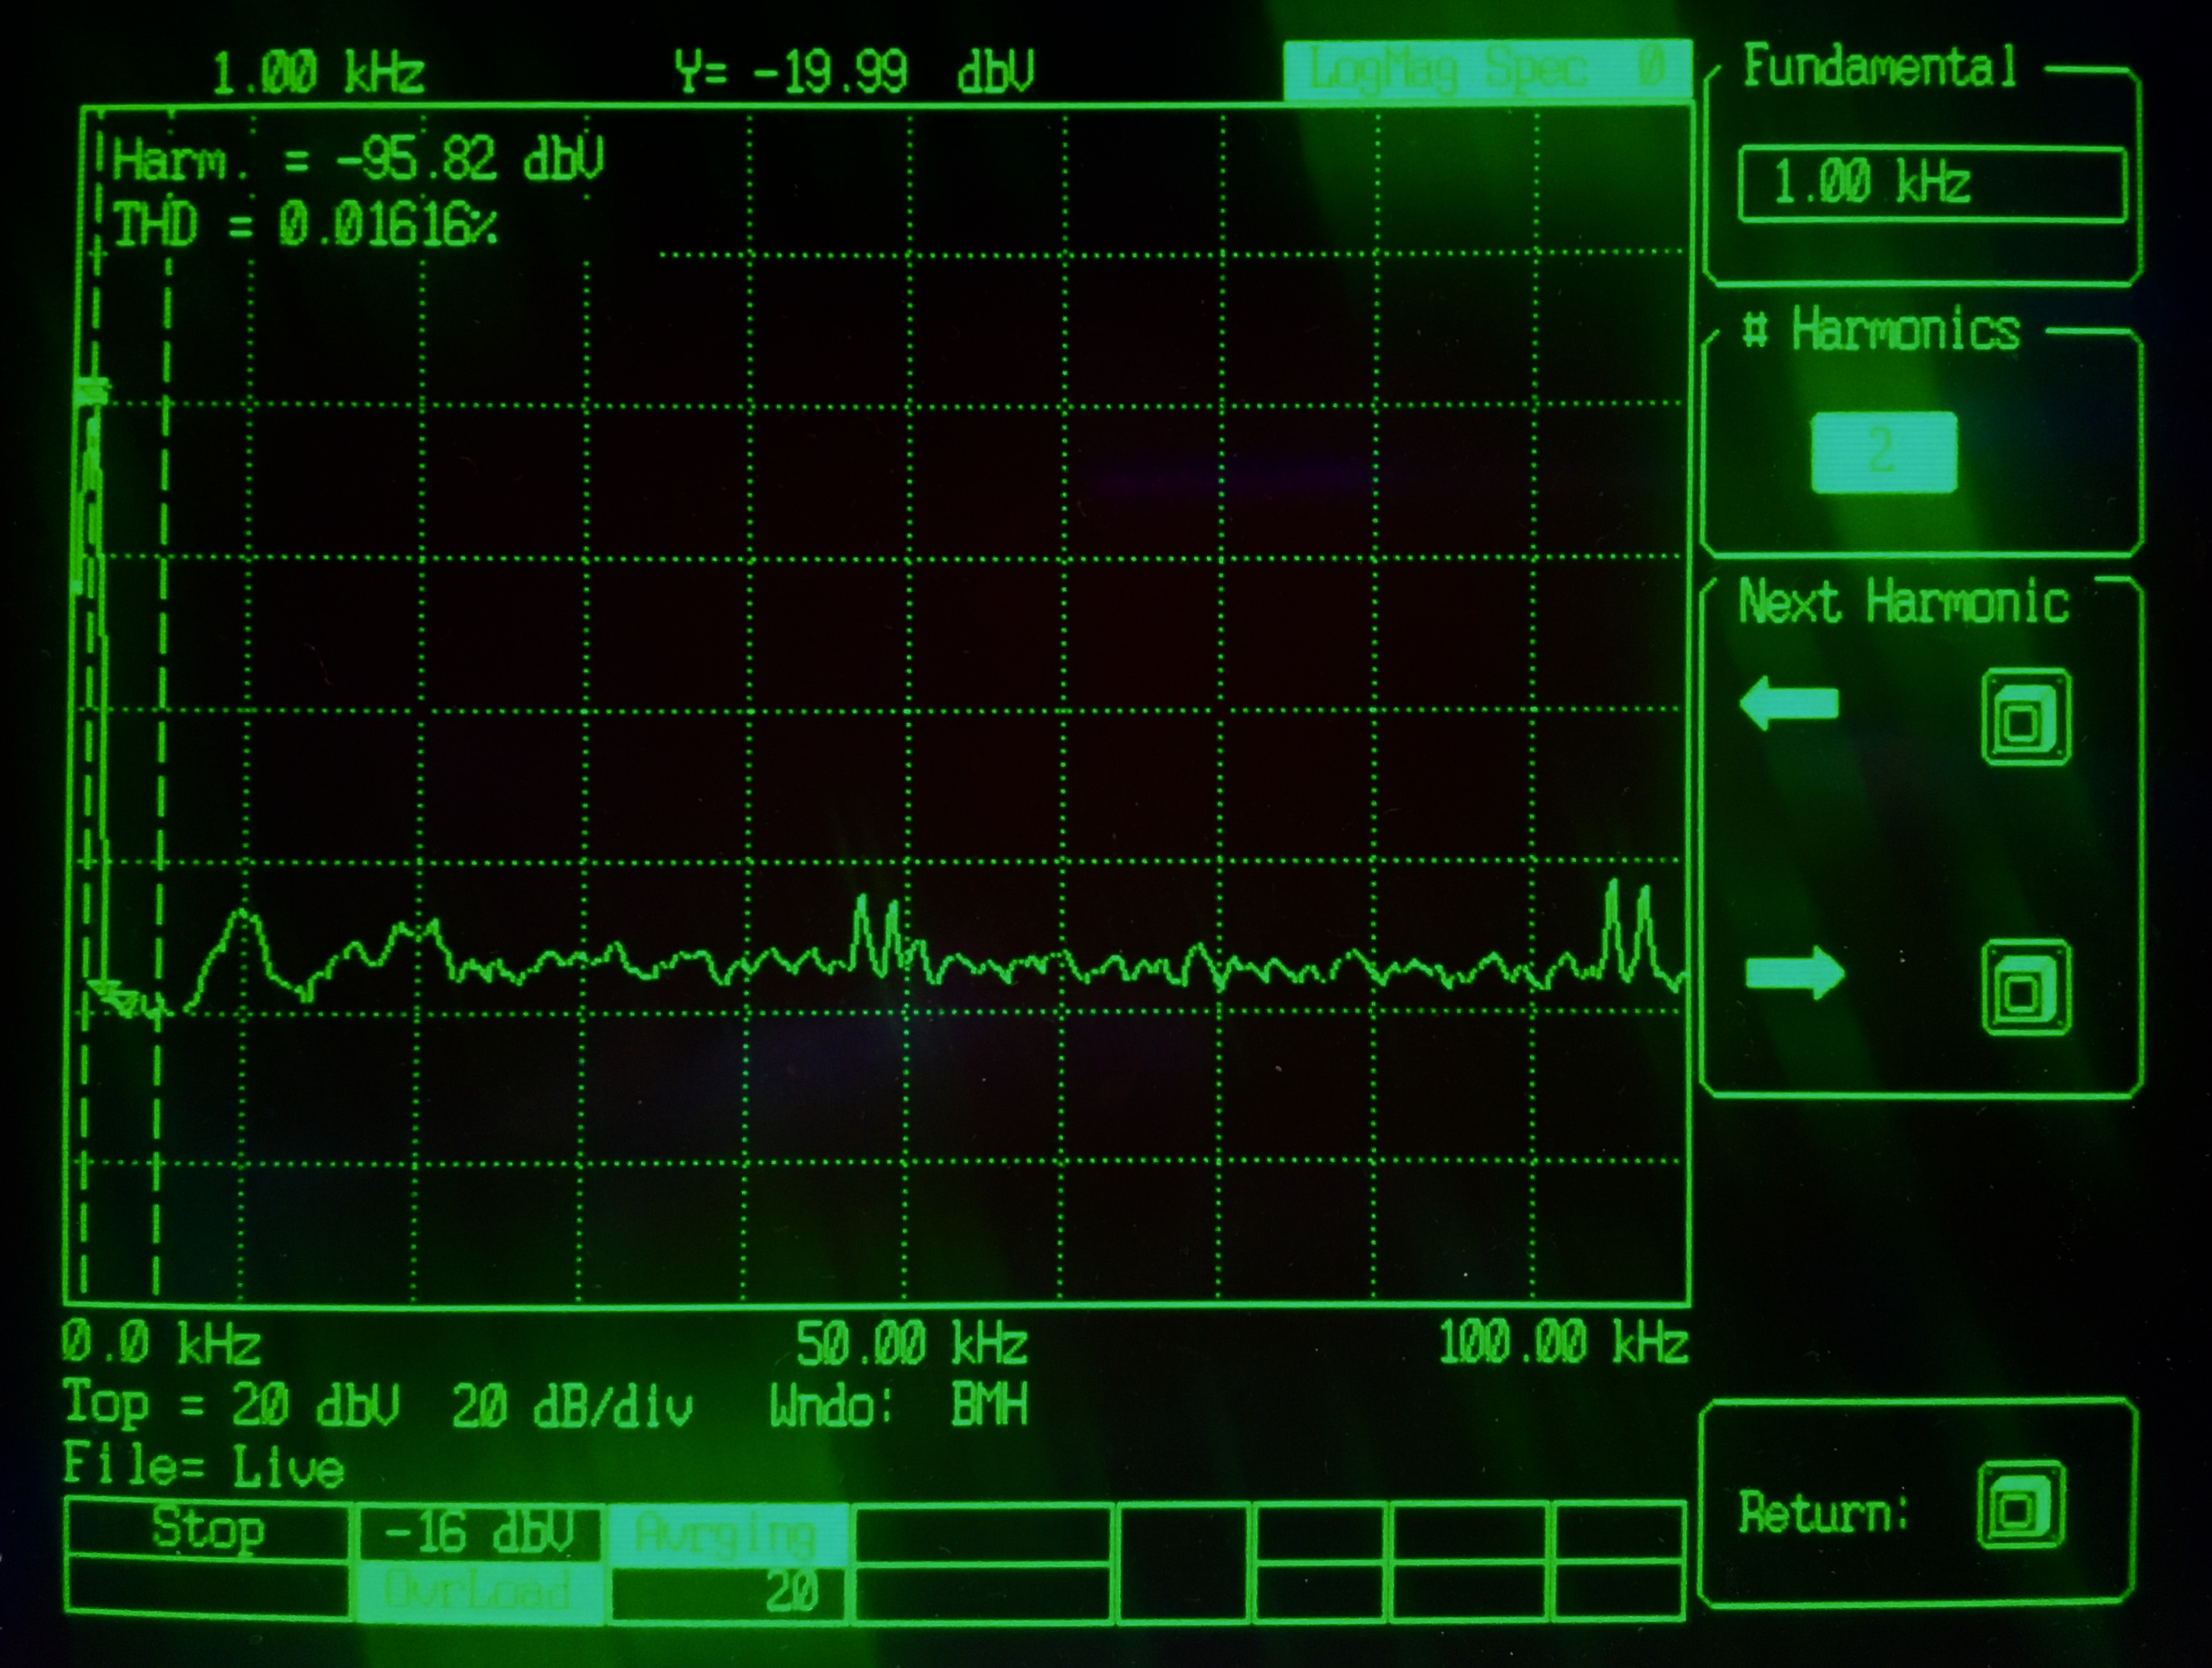
\includegraphics[scale=0.1]{../graphics/THD.jpg}
 \caption{Die gemessene Total Harmonic Distortion mit dem Stanford SR770 FFT Network Analyzer}
\label{fig:thd}
\end{center}
\end{figure}

Eine Messung mit dem Stanford SR770 FFT Network Analyzer \ref{fig:thd} ergab eine THD von 0.016\% unter Berücksichtigung von 2 Harmonischen.
Um jedoch die Messung zu verifizieren wird eine zweite Messung mit dem AD2 \ref{fig:thdAD2}  durchgeführt. Diese ergab eine THD von -75.7744dB, was ebenfalls 0.016\% entspricht. Betrachtet man fünf harmonische Vielfache erhöht sich die THD nur leicht auf 0.021\%. Das heisst die ersten fünf harmonische Vielfachen des 1kHz Sinus tragen nicht einmal ein tausendstel zum übertragenen Signal bei.

\begin{figure} [H]
\begin{center}
 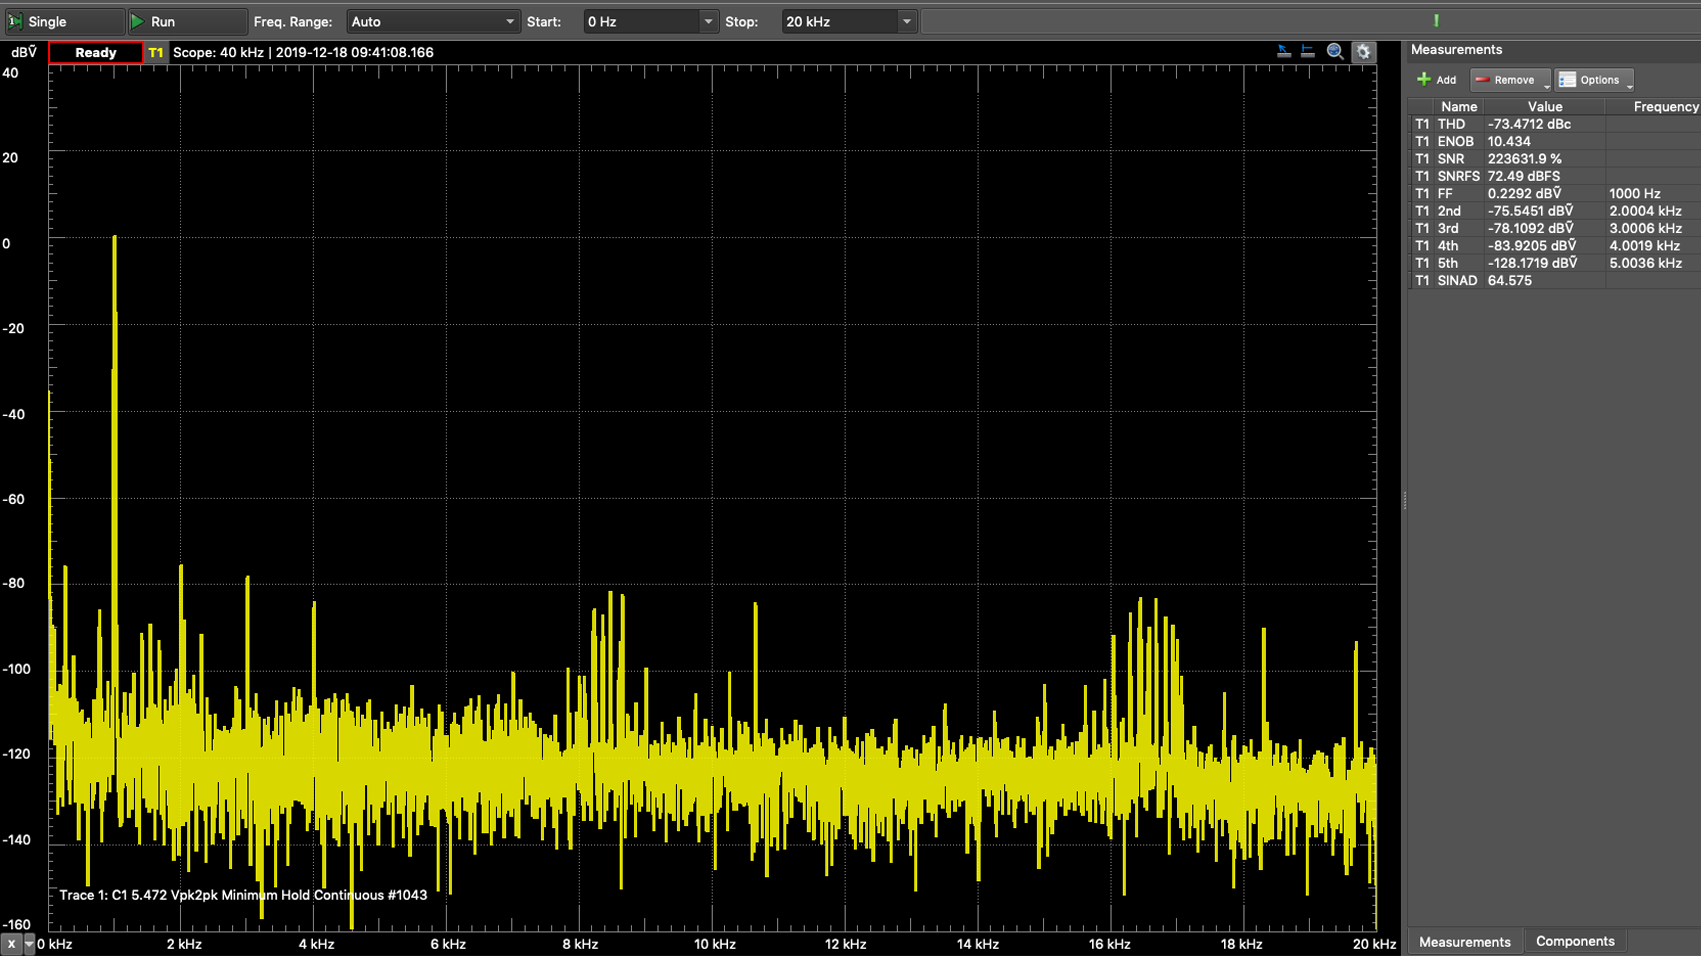
\includegraphics[width=\textwidth]{../graphics/THD_LineINOUT_Kopie.png}
 \caption{Die gemessene Total Harmonic Distortion mit dem Analog Discovery 2 von Digilent}
\label{fig:thdAD2}
\end{center}
\end{figure}

